\chapter{Metodologi Penelitian}

Berdasarkan rumusan masalah, ruang lingkup penelitian, serta batasan penelitian yang sudah dibahas pada bab sebelumnya, berikut ini adalah metodologi penelitian yang penulis gunakan:

\begin{figure}
    \centering
    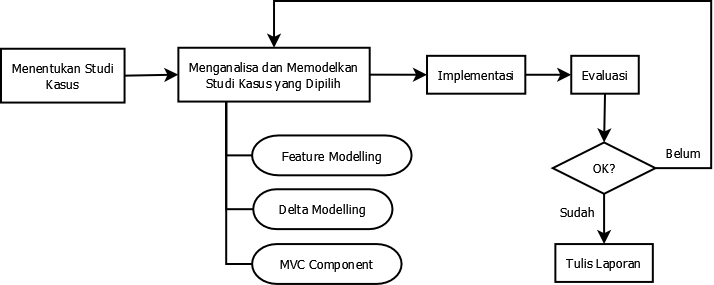
\includegraphics[width=0.8\textwidth]
        {img/alur-penelitian.png}
    \caption{Rencana Penelitian}
\end{figure}

\noindent
Di awal penelitian, penulis akan melakukan fiksasi studi kasus yang akan digunakan dalam penelitian ini. Setelah proses fiksasi studi kasus, berikutnya penulis akan melakukan analisis studi kasus tersebut serta memodelkan solusi yang akan dibuat. Hasil dari proses analisi ini adalah berupa diagram \textit{feature modelling}, \textit{delta modelling} dan daftar komponen-komponen MVC yang akan dibuat. Langkah selanjutnya adalah mengimplementasikan model yang sudah dibuat agar nantinya dapat diperoleh sebuah \textit{framework} ABS MVC yang utuh sesuai dengan hasil analisa dan pemodelan dari studi kasus pada tahap sebelumnya. langkah terakhir adalah melakukan uji kelayakan dari \textit{framework} yang selesai dibuat. Apabila \textit{framework} yang dihasilkan belum memenuhi syarat kelayakan, maka penulis akan melakukan proses analisa dan pemodelan kembali untuk dapat memperbaiki framework yang ada.

%---------------------------------------------------------
\section{Fiksasi Studi Kasus}
%---------------------------------------------------------
Pada tahap ini penulis akan menentukan studi kasus seperti apa yang akan digunakan dalam penelitian ini. Studi kasus yang digunakan pada tahap ini bukanlah sebuah studi kasus yang komperhensif melainkan hanya digunakan untuk mensimulasikan strategi pengembangan SPL berbasis web dengan menggunakan framework yang telah dibuat. Dalam penelitian ini penulis akan membuat sebuah aplikasi keuangan berbasis web yang ditujukan untuk mengelola dana donasi sebuah lembaga kemanusiaan. Adapun fitur-fitur yang akan dibuat dalam studi kasus kali ini antara lain adalah:

\begin{enumerate}
    \item \textit{Create, Retrieve, Update} dan \textit{Delete} (CRUD) data dotanur lembaga.
    \item CRUD data program sosial lembaga.
    \item Laporan pengeluaran dana donasi.
    \item Laporan pemasukan dana donasi.
\end{enumerate} 

%---------------------------------------------------------
\section{Melakukan Analisa dan Pemodelan}
%---------------------------------------------------------
Pada tahap ini penulis akan mencoba menganalisa studi kasus yang dipilih terkait dengan fitur-fitur apa saja yang harus dibuat, variasi fungsi seperti apakah yang dapat dibuat dari studi kasus tersebut, serta skema partisi yang akan digunakan dalam tahap pengembangannya. Setelah selesai melakukan analisa, berikutnya adalah memodelkan studi kasus tersebut berdasarkan hasil analisa yang diperoleh sehingga nantinya akan dihasilkan sebuah \textit{feature model}, \textit{delta model}, dan daftar komponen MVC yang harus dibuat untuk studi kasus tersebut.

%---------------------------------------------------------
\section{Implementasi}
%---------------------------------------------------------
Pada tahap ini penulis mulai mengimplementasikan model-model yang sudah dibuat pada tahap sebelumnya. Proses implementasi yang dimaksud adalah mulai membuat kode-kode ABS yang dibutuhkan sesuai dengan model yang telah dibuat serta membuat \textit{web server} sederhana yang nantinya akan digunakan untuk menguji coba SPL berbasis web yang dihasilkan.

%---------------------------------------------------------
\section{Evaluasi}
%---------------------------------------------------------
Pada tahap ini penulis akan melakukan evaluasi terhadap SPL berbasis web yang telah berhasil dibuat pada tahap implementasi. Salah satu faktor yang dinilai pada tahap evaluasi ini adalah terkait kesesuaian aplikasi dengan model atau rancangan yang sudah ditentukan pada tahap analisa dan pemodelan. Apabila hasil evaluasi dari aplikasi yang dibuat belum memuaskan, maka harus ada proses analisa dan pemodelan kembali untuk melihat apakah ada bagian yang harus direvisi atau tidak. Jika hasil evaluasi aplikasi sudah memuaskan maka selanjutnya adalah menuliskan laporan penelitian. \\

\noindent
Berikut ini adalaha syarat kelayakan yang akan dijadikan parameter dalam tahap evaluasi ini:

\begin{enumerate}
    \item Apakah \textit{framework} yang dihasilkan sudah sesuai dengan kaidah MVC yang berlaku? (sesuai dengan yang ada pada studi literatur)
    \item Apakah \textit{framework} yan dihasilkan dapat diintegrasikan dengan \textit{feature modelling} dan \textit{delta modelling} pada ABS?
    \item Apakah \textit{framework} yang dihasilkan sudah dapat mengasilkan sebuah \textit{complete product} SPL berbasis web? (dapat dijalankan)
\end{enumerate}

%---------------------------------------------------------
\section{Penulisan Laporan}
%---------------------------------------------------------
Pada tahap ini penulis akan menuliskan laporan penelitian dan menarik kesimpulan yang diambil dari penelitian yang sudah dilakukan serta memaparkan temuan-temuan yang diperoleh selama melakukan penelitian.